% Group: 	2
% Name: 	Coding Pharaohs
% Document: 	SDD incomplete first draft
% Author:	Matthew Nestor
% Date:		Tuesday September 10 2013

\documentclass[11pt, a4paper,titlepage]{article}
\usepackage[pdftex]{graphicx}
\topmargin -1cm

\begin{document}
 \begin{titlepage}
 \centerline{\small The University of Adelaide}
 \centerline{\small COMP SCI 3006/7015 Software Engineering and Project}
 \vspace{5cm}
 \centerline{\bf \huge Software Design Document}
 \centerline{\bf \huge (SDD)}
 \vspace{0.5cm}
 \centerline{\LARGE for}
 \vspace{0.5cm}
 \centerline{\bf \huge Road Closure Marking}
 \centerline{\bf \huge Robot}
 \vspace{1cm}
 \centerline{Version 0.1}
 \vspace{1cm}
 \centerline{Prepared by Group 2}
  \end{titlepage}
 \tableofcontents
 \newpage
 {\bf \large Change History}\newline

 \begin{tabular}{| c | c | l |}
  \hline
  Date & Version & Reason for Change \\
  \hline
  10th Sept & 0.1 & Initial draft \\
  \hline
 \end{tabular}

 \newpage
  \section{Introduction}
    \subsection{Purpose}
    \subsection{Scope}
    \subsection{References}
    \subsection{Overview}
    \subsection{Constraints}
     \vspace{3cm}

 
  \section{System Overview}
   \vspace{3cm}

  \section{System Architecture and Components Design}
    \subsection{Architectural Description}
    \begin{itemize}
     \item Architectural Pattern: Pipe and Filter
     \item Control Style: Centralised (Manager Model)
    \end{itemize}

    \subsection{Component Decomposition Description}
    \begin{itemize}
     \item Object Oriented Style
    \end{itemize}
    
    \subsection{Detailed Components Design Description}
    \subsection{Architectural Alternatives}
    \subsection{Design Rationale}
    
  \newpage
  \section{Data Design}
    \subsection{Database Description}
    \subsection{Data Structures}
  
  \newpage
  \section{Design Details}
    \subsection{Class Diagrams}
    %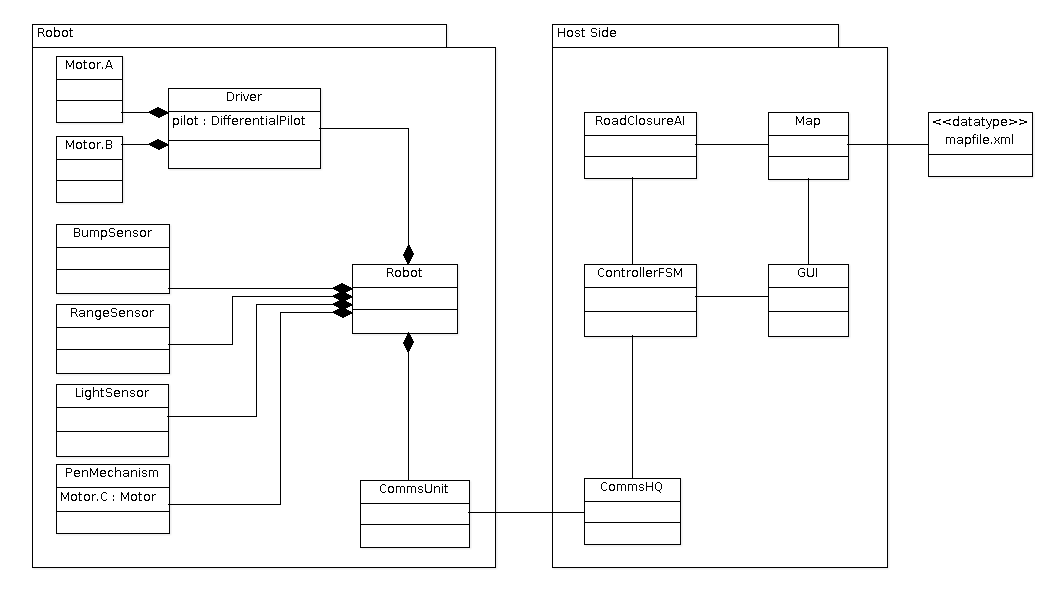
\includegraphics[height=10cm,width=20cm,angle=90]{UML/softwareArch.png}
    \subsection{State Diagrams}
    %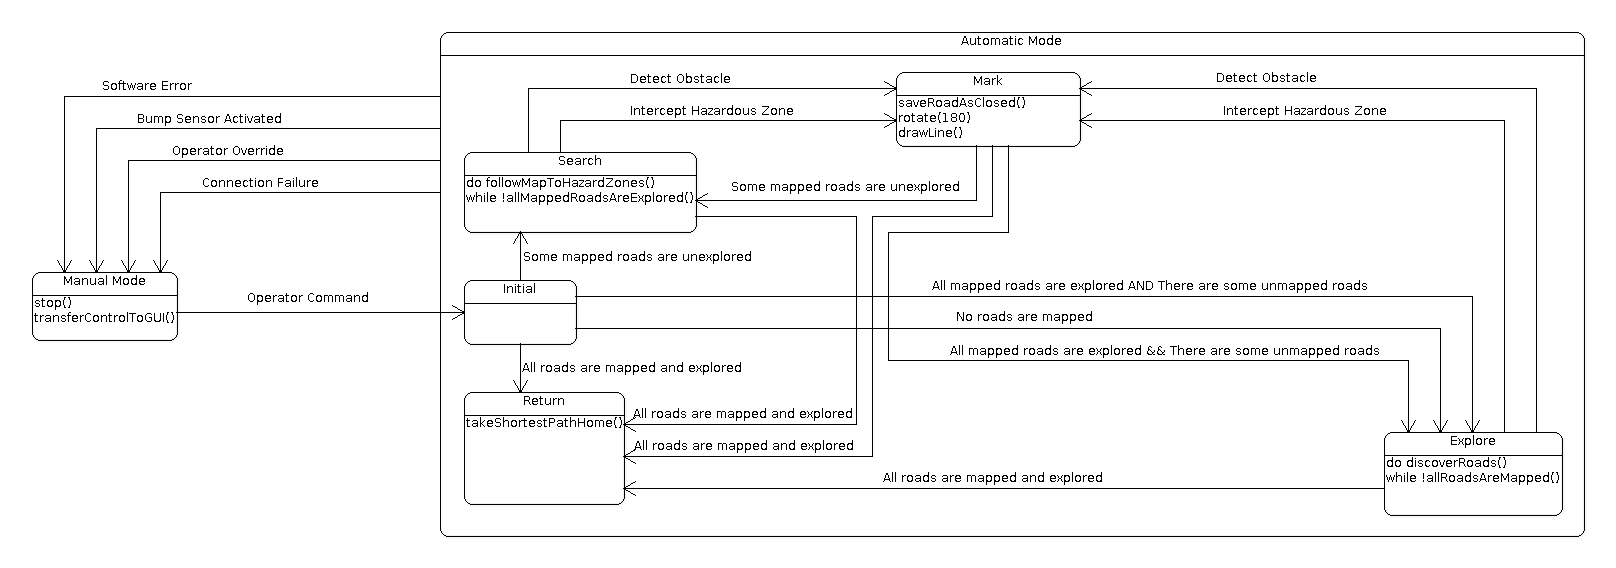
\includegraphics[height=10cm,width=25cm,angle=90]{UML/softwareFSM.png}
    \subsection{Interaction Diagrams}
  
\newpage
\section{Human Interface Design}

\subsection{Overview of the User Interface}

According to SRS, a GUI is essential on the PC side for the user to implement the following activities:
\begin{itemize}
\item The operator can establish communication with the robot by using GUI to manipulate the Bluetooth device.
\item The operator is able to manually control and monitor the robot's movement by operating a set of buttons and seeing a map panel.
\item The operator has the authority to command the robot to perform the AI mode by clicking buttons on the GUI, and then notice the robot status by receiving a bunch of messages showed on the GUI.
\item The operator is able to stop the movement of the robot by using the emergency stop button in the GUI whenever an emergency occurs.
\item The operator can control the robot in some perticular extents to ensure the optimised task completion of the robot through the GUI, e.g. monitoring the battery life or adjusting the speed of robot.
\end{itemize}

\noindent The design of the GUI is in accordance with SRS purposing a simulation of the real world to provide visibility of system status to user. The GUI should be consistent and standardised to ensure user control freedom, error provention, safety precaution, and risk handling. To achieve the ease of using for users, the GUI should be flexible, efficient of use, aesthetically friendly, minimalist design, and smooth for control flow. \\
\\
The development of the GUI follows the process below:
\begin{enumerate}
\item Relevant data gathering \\
Infer information for GUI from requirements; analyse user habits, contorl flow, and environments; derive from initial strategy and data presentation.
\item Prototypes \\
Create prototype based on the results of last phase.
\item Revisions \\
Show the prototype to stakeholders (the group and client) for feedbacks and recommendations. If passed move to next stage otherwise design a new prototype or modify the existed prototype.
\item Documentation \\
Create User Manual for the GUI.
\item Final review \\
Final demonstration for assessment.
\end{enumerate}
\subsection{Detailed Design of the User Interface}

According to the ``User Interface'' section of SRS, the GUI should consist of four parts:
\begin{enumerate}
\item Command buttons allow the operator to control the movement or change the status of the robot, including:
\begin{enumerate}
\item forward. Press once and the robot will continue moving forward.
\item backward. The same as forward.
\item left. Rotate the robot ninty degrees to left.
\item right. Rotate the robot ninty degrees to right.
\item connect. Establish the connection from PC to robot.
\item disconnect. Disconnect the bluetooth connection between PC and robot.
\item mark road closure. Command the robot to manually mark road closure.
\item start automatic mapping. Enable the AI mode of the robot to automatically explore the map.
\item return to base. Make the robot return to the starting position.
\item stop. The emergency stop for the robot.
\end{enumerate}
\item Robot information area contains the information in relation to the robot's status, including:
\begin{enumerate}
\item robot name.
\item battery level. Display the current battery level of the robot.
\item connection status. Display the status of Bluetooth connection using ``on'' and ``off''.
\item message. A textfield shows the messages sent by the robot including values of sensors, status of the robot, and warnings.
\end{enumerate}
\item Map area \\
A panel in the GUI to diaplay the current map. All objects defined in the DTD will be showed on the map, including roads, road intersections, obstacles, disaster area, closure, and unexplored area. The current location of the robot and traversed path by the robot would also be showed in the map.
\item List menu. \\
A menu that allows the operator to save and reload the map in the form of XML file in the format specified by the DTD by clicking items in the list menu.
\end{enumerate}

\noindent The display space for mapping is the major core component of the GUI, and it shall be maximised. All other functions except for the list menu are located at left-hand-side of the display window with a constant width so the display of map can be enlarged for larger screen sized window. The menu list is put on the top left of the window as a button on the top tool bar. The whole menu will emerge after a click on the menu button. Inside the menu list the user will see menu items to deal with the XML file. \\
\\
The functions of GUI, which were designed upon the requirements elicitation, are outlined as following:
\begin{enumerate}
\item R01 and H02: Manual Control of the robot: \\

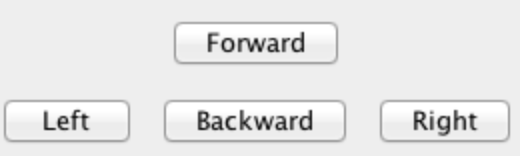
\includegraphics[width=11.5cm]{images/3.png}
\vspace{15pt}

\item R02-03: Map saving and loading: \\


\includegraphics{images/5.png}
\vspace{15pt}

\item R07: Road closure marking: \\


\includegraphics{images/1.png}
\vspace{15pt}

%\newpage
\item H01: The whole GUI: \\


\includegraphics[width=11.5cm]{images/2.png}
\vspace{15pt}

\item H04: Emergency stop: \\


\includegraphics{images/4.png}
\vspace{15pt}

\item Other attributes stated in other descriptions of SRS: \\
\\
AI mode: \\


\includegraphics{images/6.png}
\vspace{15pt}
\\
\\

Status: \\


\includegraphics{images/8.png}
\vspace{15pt}

Connection: \\

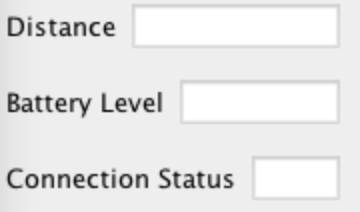
\includegraphics{images/7.png}
\vspace{15pt}

\newpage
\item The display of the map: \\

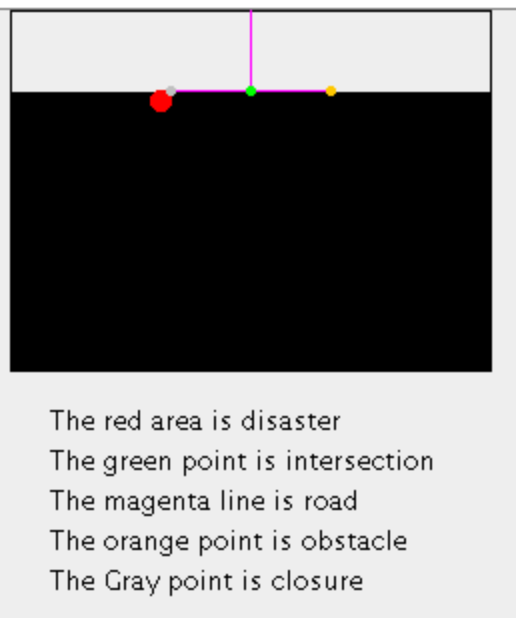
\includegraphics{images/9.png}
\vspace{15pt}
\end{enumerate}

\noindent The functions that have already been defined in SRS but not been implemented yet in the GUI, are outlined as following:

\begin{enumerate}
\item M01: Display the taversed path by the robot in map panel.
\item H03: Display the current position of robot in map panel.
\item H06: A textfield on the GUI to show messages such as alert message.
\item SA01: A speed bar on the GUI to adjust the speed of the robot. The speed should be within a safe speed.
\item Other function that was not described in SRS: Zoom feature for the map.
\end{enumerate}
    
  \newpage
  \section{Resource Estimates}
   \vspace{3cm}
  \section{Definitions, Acronymns and Abbreviations}
  
\end{document}
